

\section*{Project II: Genome binning of viral entities from bulk metagenomics data}

In this project we expanded the scope of genome binning to viruses in metagenomics using VAMB as our binning engine. We trained a RF model using paired metagenomes and metaviromes to filter and extract putative viromes from metagenomics (Figure \ref{fig:RF_phamb}). Applying the trained RF model to any binned metagenome aids in the delineation of bacterial MAGs and viral MAGs (vMAGs), which can be followed up with exploration into host-viral dynamics and viral gene contributions and dissemination (Figure \ref{fig:RF_phamb}). Finally, we benchmarked viral genome recovery with a binning approach using synthetic CAMI generated datasets and three metagenomic datasets COPSAC, Diabimmune and HMP2 IBD.


\begin{figure}
  \begin{center}
    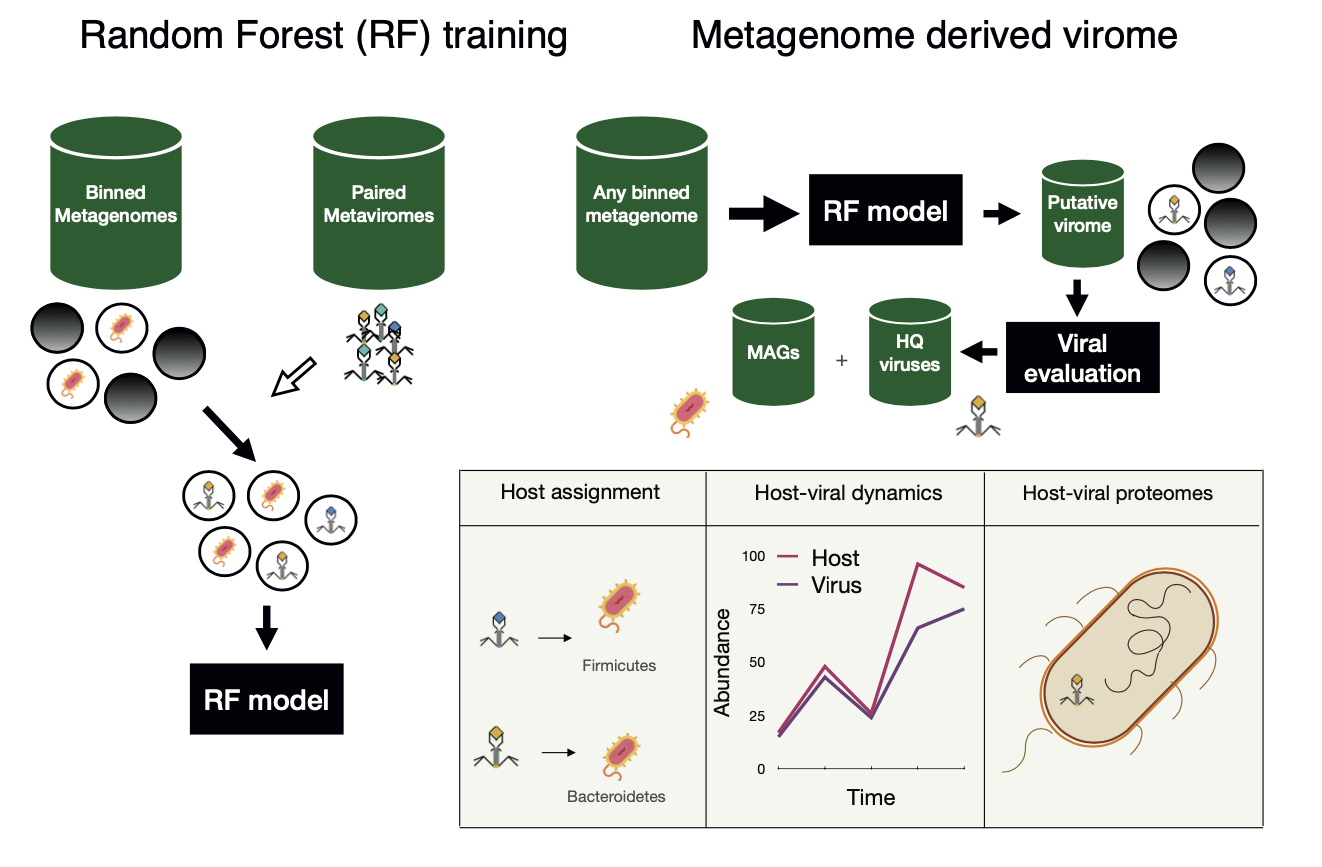
\includegraphics[scale=1,width=1\textwidth]{pictures/RF_phamb.png}
  \end{center}
  \caption[VirusTimeline]{Random Forest (RF) modeling was performed on binned metagenomes paired with metaviromes. The trained RF model can be applied to any binned metagenome for predicting the putative virome in which high-quality (HQ) viruses can be identified and combined with bacterial MAGs. Identification of virus host affiliation enables analysis into host-viral abundance dynamics and the functional space shared between bacterial host and viruses.
  }
  \label{fig:RF_phamb}
\end{figure}

\noindent
One of the first facets of the paper to be discussed is the motivation for viral binning. Binning of bacterial MAGs has been in development for many years, why not viruses?

\subsection{To bin or not to bin?}

To achieve an absolute number on the improvement on viral genome quality gained with binning, we tallied the number of viruses recovered as single contigs and viral bins by genome quality tiers. We were able to recover up to 210$\%$ additional high-quality (HQ) viral genomes compared to using a single contig virus approach. To ensure a fair comparison, we investigated the exact same set of contigs in every dataset with and without binning. In addition, we found that binning enabled recovery of up to 36$\%$ of HQ viral populations found in the metavirome directly from paired bulk metagenomics data. Furthermore, 47$\%$ additional HQ viral populations were discovered in bulk metagenomics and not in the metavirome. Here, a likely explaining factor is viral sampling bias as a result of sample preparation, since metavirome preparation concentrates smaller viruses and predominantly viruses in a lytic stage and not integrated in bacteria \cite{Roux2019-dc}. The surprisingly high intersection (36$\%$) of viruses in metagenomics with and without viral-enrichment , which has been estimated to 8.5-10$\%$ in another study \cite{Gregory2020-gu}, suggests a great potential to conduct virome analysis based on bulk metagenomics.\\

\noindent
A major worry with binning is the risk of including contigs from other sources of species such as genome bin contaminants. We benchmarked the degree of contamination to an average of 2.55$\%$ of the viral bin genome in base pairs not aligning to the virus of reference, which equals a genome purity of 97.45$\%$ on average. This benchmark was also performed on synthetic datasets where the average genome purity was 94.5$\%$. Evidently, viral binning with our methods is not a perfect process and does pose some risk for virus contamination, although contaminating sequences may be removed during bin post-processing. Binning is also a process which disregards the correct order of contigs in a genome as it merely groups contigs together that belong to the same genome. This might not be desirable if a researcher is interested in the order of virus gene transcription during infection of a bacterial host. For instance, phage encoded anti-defense proteins that counteract bacterial defense systems are suggested to be phage early genes \cite{Gao2022-ux}. The correct order of phage genes annotated in a genome can therefore be critical for determining novel anti-defense genes that are expressed prior to defense system activators such as portal and terminase proteins, which are recognised and activate antiviral defense systems \cite{Gao2022-ux}.\\ 

\noindent
With the goal of virus discovery in mind on new or old metagenomic datasets, we have shown that binning improves identification of higher quality virus genomes. On the contrary, if a researcher's focus is to perform massive virus mining across hundreds of thousands of assembled metagenomic contigs on NCBI, corresponding to single-contig identifications, binning is not a technically feasible solution at this moment as it requires a contig x sample matrix. Including $>$20.000 of samples with several millions of contigs results in an astoundingly big matrix with intense demand for computational processing and memory allocation. However, for single datasets such as a new metagenomic dataset from a cohort of patients, the unsupervised clustering algorithm built into VAMB provides strain-like viral clusters simultaneously with bacterial MAGs. As such, the genome of an abundant virus in a patient can be tracked and compared across multiple samples, if longitudinally sampled, simultaneously with the predicted bacterial host. We illustrated for the HMP2 dataset that the VAMB-clusters produced for crAss-like virus genomes were accurately differentiated on a high taxonomic level, which we illustrated in a phylogenetic tree (Figure \ref{fig:crasstree}). Essentially, we found that viral binning across a cohort enables precise clustering of viral populations with high intra-VAMB-cluster ANI ($>$97.5$\%$) that can be leveraged for longitudinal or cross-sectional viral genome comparison studies.

\begin{figure}
  \begin{center}
    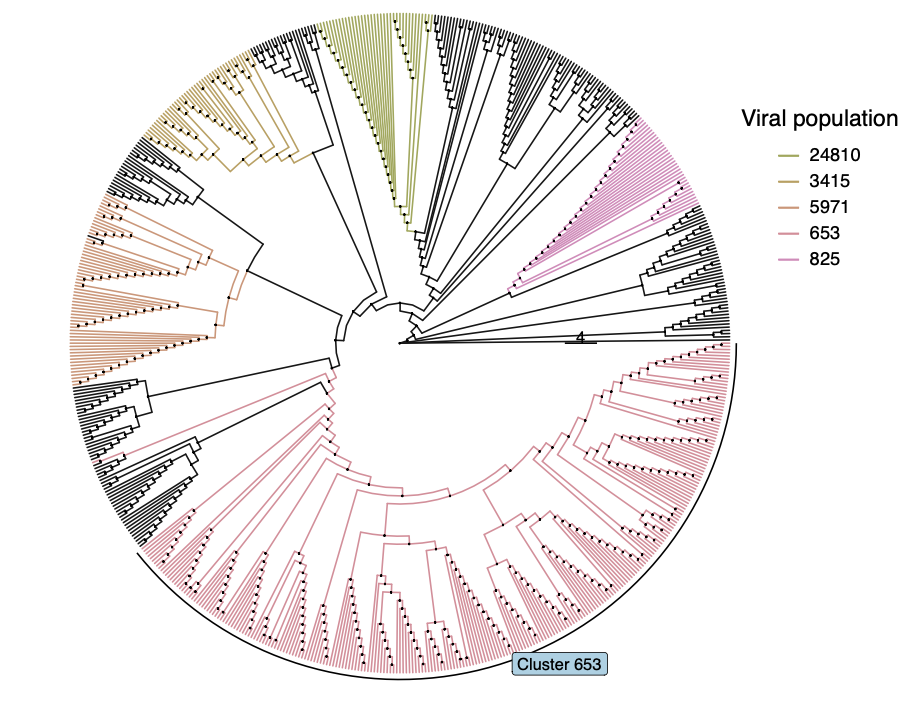
\includegraphics[scale=1,width=1\textwidth]{pictures/crasstree.png}
  \end{center}
  \caption[VirusTimeline]{Cladogram based on a phylogenetic tree of crAss-like virus genomes colored and named by VAMB-cluster.
  }
  \label{fig:crasstree}
\end{figure}

\subsection{What we learned about the virus functional potential}

Based on the current tools available for annotating protein domains, we established that the viral protein-coding genes in HMP2 exhibited high prevalence of core viral proteins related to structure (capsid, tail, head etc.) and integrase enzymes for integration into host chromosomes. In addition, we also found a high frequency of reverse-transcriptase (RT) domains in viral proteins. RT domains are increasingly identified in multiple gene configurations that go way beyond the RTs’ role as a retro-viral transcriptase necessary for RNA-virus replication. RT domains have been identified in numerous prokaryotic anti-phage defense systems, such as restriction modification enzymes and abortive infection mechanisms \cite{Toro2019-zp} and in diversity generative regions (DGRs) \cite{Roux2020-mr}. In order to circumvent bacterial defense systems and exclude other viral competitors, phages also encode prokaryotic defense systems such as anti-viral systems \cite{Rousset2022-sn}. Thus, the high frequency of annotated RT domains indicates the potential abundance and importance of these genetic systems in the bacterial-phage arms race. Future studies should leverage new bioinformatic tools to annotate the presence of anti-phage systems in bacteria \cite{Payne2021-xt} and phages to further understand intricate interactions in complex environments like the human gut. Furthermore, we also identified proteins in phage genomes with TonB plug and TonB receptor domains that encode established immune stimulating epitopes \cite{Graham2018-me}. This finding underscores the presence and potential phage-driven distribution of epitopes that may stimulate host immune cells and contribute to gut immune stimuli. A completely different perspective is cross-reactivity with phage-encoded epitopes that activate host T-cells through MHC-1 receptors via “molecular mimicry” \cite{Fluckiger2020-ay}. Studies on the commensal epitope landscape should strive to recognise the presence of epitopes in bacteria and viruses, as the abundance of both entities may impact host immune activity during health and disease.

\subsection{The future of virome analysis without viral enrichment}

One of the major motivations for benchmarking virus recovery with binning in the first place was to investigate virome analysis for datasets where whole-virome sequencing is not available. To evaluate the methods' utility, we applied it to a massive public metagenomic dataset, the HMP2, from which no virome characterisation had been described before. Here we identified 3,625 viral populations consisting of 16,358 viral bins (Medium-quality or better). We have illustrated that virus-binning is feasible and quite valuable, thus future efforts in binner-development will likely improve upon these numbers by harnessing better computational models trained on better and larger datasets. Nevertheless, can we imagine a future without the need for binners?\\ 

\noindent
Certainly, 3rd generation (long-read) sequencing technologies such as Nanopore and PacBio can produce long-reads which improve the assembly and binning of genomes from metagenomics \cite{Moss2020-ot,Sereika2022-ii}. Furthermore, recent results have shown that combining short and long reads increased the number and genome-quality of viruses in marine environments compared to illumina sequencing (short read) alone \cite{Zaragoza-Solas2022-ky}. These results may be a primer for the 3rd generation sequencing coming of age where long-reads can capture viruses in whole sequences, which ultimately alleviates assembly issues caused by repeat and low-coverage regions found in virus genomes \cite{Sutton2019-zv}. However, the recurring issues with 3rd generation sequencing comprises higher base-calling error rate and frequency of insertions and deletions (indels) \cite{Delahaye2021-ys}. Combining long-reads and short-read sequencing has been the common strategy to deal with long-read errors, where short-reads are used to correct errors in assembled sequences \cite{Wick2017-as}. Yet, recent Nanopore technology has shown to bridge the gap in terms of price and sequencing accuracy while also increasing the number and quality of recovered prokaryotic genomes \cite{Sereika2022-ii}. So, where do we stand in terms of long-read sequencing of viruses in bulk metagenomics? Recent studies have explored the benefits of combining 2nd and 3rd generation sequencing \cite{Zaragoza-Solas2022-ky,Yahara2021-jx} and shown that long-reads captured additional viral diversity but also illustrated that long-reads with PacBio sequencing only captured few HQ viruses \cite{Zaragoza-Solas2022-ky}. Thus, hybrid assembly combining short and long-reads seems to be a promising strategy for exploring viruses in bulk metagenomics at this point in time. At the very least, improved recovery of MAGs with long-read sequencing may strengthen identification of complete proviruses.

\subsection{Frameworks for benchmarking virus completeness, where credit is due}

In 2022, gut ecologists have access to reliable and trusted frameworks for identifying and annotating virus genomes, both \textit{de novo} and by reference-based approaches. An assembled putative virus sequence is automatically gene-annotated using a wealth of finely curated virus marker databases and simultaneously aligned to a massive collection of viruses composed of hundreds of thousands of genomes \cite{Nayfach2021-yf}. Thus, phage-genomic research has indeed rocketed since the year of 2019 when we initiated the planning of a benchmark on viral genome binning based on bulk metagenomics assemblies. Programmes like Virsorter and Virfinder did exist but lacked features for referencing viruses in the space of known biodiversity or scoring genome-completeness to address whether a virus genome was complete or a fragment. Therefore we designed our benchmark strategy based on paired metaviromes with \textit{bona fide} assembled viruses, which provided a sensible starting point for calculating one-to-one (viral-bin to virus) comparisons. Alas, two convenient bioinformatic tools were released in 2020, CheckV and VIBRANT, which brought new standardized measurements of virus quality such as completeness and contamination while simultaneously referencing a grand catalog of viral biodiversity. The extent to which binning can be used for recovering viruses in metagenomics could not have been explored so extensively without research efforts from other research-groups such as the Microbiome Data Science Group at JGI-DOE and Anantharaman-lab, to whom we are grateful. A background and blogpost about the article and research was further published in Nature’s microbiology community forum \footnote{\url{https://microbiologycommunity.nature.com/posts/microbiome-analysis-of-viruses-is-more-accessible-than-ever}}. In addition, we were fortunate that a science journalist at the danish newspaper Politiken (Appendix \ref{appendix:politiken}) found our article relevant for a story on combating antimicrobial resistance using phage cocktails \footnote{ \url{https://politiken.dk/viden/Viden/art8735714/Praksissen-var-ellers-g\%C3\%A5et-i-glemmebogen-i-Vesteuropa-men-nu-har-forskere-for-alvor-f\%C3\%A5et-\%C3\%B8jnene-op-for-tarmbakterierne}}.\\ 

\noindent
In order to define future phage cocktails that can target and kill bacterial culprits, the relevant and specific viruses have to be discovered first, which is what our methods can support. The next question we phrased was: what metagenome and context would benefit from virus discovery and virome analysis? We had an established starting point for virome analysis in bulk metagenomics, but where to begin? A general topic of interest is the influence of age on the human microbiome and its development over time, which has been investigated extensively for bacteria \cite{Stewart2018-vm,Ghosh2022-vc}. A recent study into the infant virome had revealed the turbulent development of the pioneering viral constituents and response to the maturing bacterial community \cite{Liang2020-lr}, while another mapped the development of viral families over time from infant to elderly \cite{Gregory2020-gu}. Interestingly, only a couple of studies have investigated the age-dependent effects on the virome and by no means the extreme end of human longevity.